\documentclass[oneside,UTF8,AutoFakeBold]{buaathesis}



\schoolname{北京航空航天大学计算机学院}
\title{硕士学位论文中期检查报告}
\papertitle{基于神经网络的语言模型的性能优化研究}
\specialty{计算机科学与技术}
\studentnumber{SY1506330}
\researcharea{自然语言处理}
\advisor{荣文戈}
\author{姜~~楠}
\date{2017 年 8 月 20 日}

\begin{document}

\maketitle

\tableofcontents
\newpage
\begin{table}
\center{\zihao{2}\songti\textbf{基于神经网络的语言模型的性能优化研究}}
\end{table}

\section{论文工作计划}
\subsection{论文研究目标}
近年来,随着 Internet 的兴起,互联网上的数据急剧膨胀。根据国际数据信息公司(IDC)的统计和预测,2017 年全球网络数据量已经达到1.8ZB,到2025 年,全球数据总量预计还将增长50 倍。大量无标注数据的出现,也让研究人员开始考虑,如何利用算法从这些大规模无标注的文本数据中自动挖掘规律,得到有用的信息。自从2006年, Hinton 提出的深度学习(Deep Learning, DL)概念以来\cite{hinton2006reducing},为解决这一数据爆炸问题带来了新的思路。在这之后的发展中,基于神经网络的表示学习技术(Representation Learning)开始在各个领域崭露头角。尤其在图像(Image Classification)和语音(Automatic Speech Recognition)领域的多个任务上,基于表示学习的方法在性能上均超过了传统基于特征提取的方法。

近年来,深度学习逐渐在自然语言处理中(Natural Language Processing, NLP)得到应用. 研究者提出用神经网络(Neural Network, NN) 来训练语言模型(Language Model)并进行了相关探索\cite{DBLP:conf/nips/BengioDV00}. 其中,基于循环神经网络的语言模型建模方法引起了研究者极大的兴趣[3]. 网络通过学习能够将当前词的历史信息存储起来,以词的整个上下文作为依据,来预测下一个词出现的概率,克服了n-gram 语言模型无法利用语句中长距离上下文信息的缺点. 另外,在模型训练的过程中,由于词的历史信息被映射到低维连续空间,语义相似的词被聚类,在语料中出现次数较少的词仍然能够得到很好的训练,不再需要额外的数据平滑技术. 迄今为止,采用(Recurrent Neural Network, RNN)训练的语言模型在模型困惑度(Perplexity, PPL)和识别系统的识别率上都取得了最好的效果[4]. RNN 建模方法虽然表现出极大的优越性,却以牺牲计算复杂度为代价. 若训练大规模的文本语料,则需要花费很长的时间,制约了RNN 语言模型训练效率. 为克服这一不足,文献[5] 提出了多种优化策略来降低网络的计算复杂度,如缩短模型训练周期、减少训练数据集的规模、降低训练词典的大小、减少隐含层的节点数等,这些方法都在一定程度上降低了网络的运算量,提高了模型的训练效率,但同时也牺牲了较多的模型性能. 另外,在网络结构层面上,文献\cite{DBLP:journals/coling/BrownPdLM92} 研究了一种基于分类的循环神经网络(Class-based RNN) 结构,网络的输出层被分解为两部分,增加的一部分称为分类层,从结构上降低了整个网络的计算复杂度,使得模型训练效率有了一定的提升且模型性能没有大的变化. 然而,在大词汇量连续语音识别系统中,采用此结构训练大规模语料语言模型仍需要花费大量时间. 因此,模型训练效率有待进一步优化.

\subsection{论文主要研究内容}
因此探讨研究语言模型的大词表问题,是目前理论应用到实际过程中必须要克服的问题。我们当然可以通过配置高性能服务器来暂时延缓该问题的后果,但是一旦应用到大数据集上,即使是目前最好的CPU或者GPU,仍然需要三五天时间才能训练完善。应此,在保证原有模型的准确率的目的下,如何提高模型的训练速度是我们主要讨论的内容。为此我们讨论了三个不同的方向:一种是通过采样技术(Importance Sampling)来减少必要的训练时间;一种是通过基于分类的多元分类(class-based hierarchical softmax, cHSM)来加速模型; 最后一种是采用基于树模型的多层二元分类模型(tree-based hierarchical softmax, tHSM).

同时,我们还需要针对CPU 和GPU设备分别进行探讨。因为传统的线性运算模型在流行的GPU并行运算方案中并不适用,所欲需要结合不同的运算设备分别讨论可行的方案。

\section{已经完成的工作}
基于神经网络的分布表示一般称为词向量、词嵌入(word embedding)或分布式表示(distributed representation)[116]。神经网络词向量表示技术通过神经网络技术对上下文,以及上下文与目标词之间的关系进行建模。由于神经网络较为灵活,这类方法的最大优势在于可以表示复杂的上下文。在前面基于矩阵的分布表示方法中,最常用的上下文是词。如果使用包含词序信息的n-gram 作为上下文,当n 增加时,n-gram 的总数会呈指数级增长,此时会遇到维数灾难问题。而神经网络在表示n-gram 时,可以通过一些组合方式对n 个词进行组合,参数个数仅以线性速度增长。有了这一优势,神经网络模型可以对更复杂的上下文进行建模,在词向量中包含更丰富的语义信息。神经网络模型主要包括: 传统前向传递神经网络(Feed Forward Neural Network, FFNN)、循环神经网络(Recurrent Neural Network, RNN)建模方案。

另外针对大词表问题,主要可以分为以下两种策略:基于类别的多元分类模型(class-based hierarchical softmax, cHSM)和基于二叉树的二元分类模型(class-based hierarchical softmax, tHSM),我们分别在下面详细讨论和介绍。
\subsection{完成的工作内容一: 上下文信息建模}
上下文信息建模(Context Representation)方法主要分为:前向神经网络和循环神经网络。其中前向神经网络没有考虑单词的词序信息
已经实现了基于循环神经网络的
语言模型可以对一段文本的概率进行估计,对信息检索(Information Retrieval)、机器翻译(Machine Translation)、语音识别等任务有着重要的作用。

形式化讲,统计语言模型的作用是为一个长度为$m$ 的字符串确定一个概率分布$P(w_1;w_2;\cdots;w_m)$,表示其存在的可能性,其中$w_1$ 到$w_m$ 依次表示这段文
本中的各个词。一般在实际求解过程中,通常采用链式法则(Chain Rules)将计算序列概率分解成计算其条件概率值:
\begin{equation}
\label{equ:lm}
\begin{split}
P(w_1;\cdots;w_m) &= P(w_1) P(w_2|w_1) P(w_3|w_1;w_2)\cdots P(w_i | w_1;\cdots;w_{i-1}) \\
&\cdots P(w_m | w_1;w_2;\cdots;w_{m-1})
\end{split}
\end{equation}
在实践中,如果文本的长度较长,公式.~\ref{equ:lm}右部$ P(w_m | w_1;w_2;\cdots;w_{m-1}) $ 的估算会非常困难。因此,研究者们提出使用一个简化模型:n 元模型(n-gram model)。在n 元模型中估算条件概率时,距离大于等于n 的上文词会被忽略,也就是对上述条件概率做了以下近似:
\begin{equation}
\label{equ:approx}
P(w_i | w_1;w_2;\cdots;w_{i-1})  \approx P(w_i | w_{i-(n-1)};\cdots;w_{i-1})
\end{equation}
当$n = 1$ 时又称一元模型(unigram model),公式.~\ref{equ:approx} 右部会退化成$P(w_i)$,此时,整个句子的概率为:$P(w_1;w_2; \cdots;w_m) = P(w_1)P(w_2) \cdots P(w_m)$。从式中可以知道,一元语言模型中,文本的概率为其中各词概率的乘积。也就是说,模型假设了各个词之间都是相互独立的,文本中的词序信息完全丢失。因此,该模型虽然估算方便,但性能有限。当n = 2 时又称二元模型(bigram model),代入公式.~\ref{equ:approx} 中,右部为P$(w_i|w_{i-1})$。常用的还有n = 3 时的三元模型(trigram model),使用$P(w_i |w_{i-2};w_{i-1})$ 作为近似。这些方法均可以保留一定的词序信息。

传统方法采用单词或者n元组的词频来作为n元组的概率计算方法,该方法简单有效能满足线上负载的计算需求。但是随着n的增大,模型的参数呈现指数爆炸式增长、概率计算复杂度也相应上升。目前google有在线存储的最大的9元模型,这已经是目前计算机系统存储,数据访问的极限了。

\subsection{完成的工作内容二}
上下文信息建模策略主要的思路包括: 传统前向传递神经网络(Feed Forward Neural Network, FFNN)、循环神经网络(Recurrent Neural Network,RNN)建模方案。 以下我们一一探讨。

神经网络对参数进行高度共享,因此对低频词具有天然的平滑能力。神经网络语言模型(Neural Network Language Model, NNLM) 的最早由Bengio等人在2001年提出\cite{DBLP:conf/nips/BengioDV00}, 近年来一些学者开始展开这方面的研究,并取得一系列成果,如\cite{DBLP:conf/acl/BaroniDK14,DBLP:journals/sigkdd/BellK07,DBLP:journals/pami/BengioCV13,DBLP:journals/tnn/BengioSF94}, 但总体而言, 对NNLM的研究还处在起步阶段。
具体而言,NNLM通过一个多层感知网络(Multi-Layer Perceptron, MLP)来计算公式.~\ref{equ:approx} 中概率。
\begin{figure}
  \centering
  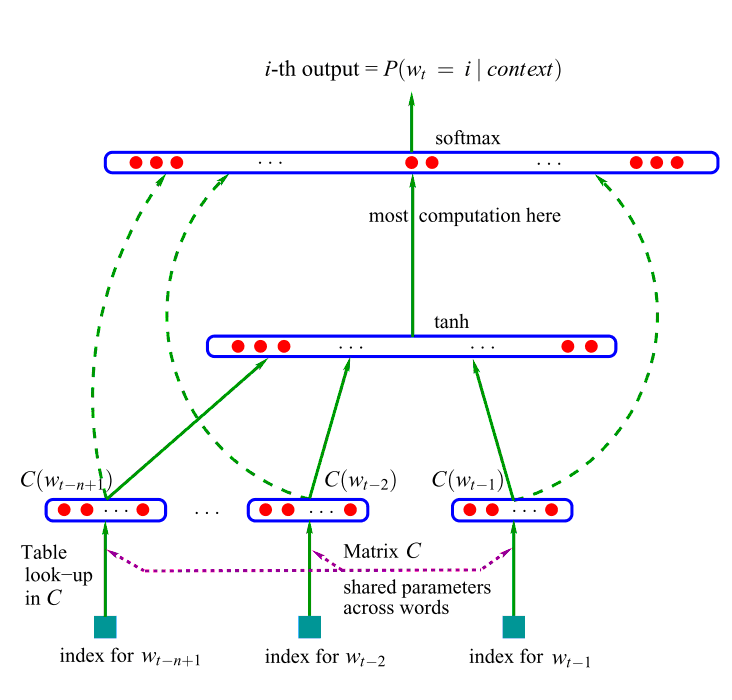
\includegraphics[width=0.6\linewidth]{./figures/nplm.png}
  \caption{前馈神经网络语言模型}\label{fig:nplm}
\end{figure}

图 \ref{fig:nplm} 给出一个典型的 NNLM 语言模型。神经网络语言模型采用普通的三层前馈神经网络结构,其中第一层为输入层。Bengio 提出使用各词的词向量作为输入以解决数据稀疏问题,因此输入层为词$w_{i-(n-1)}; \cdots;w_{i-1} $ 的词向量的顺序拼接:
\begin{equation}\label{equ:we}
  x = [e(w_{i-(n-1)}; \cdots ; e(w_{i-2}); e_{(w_{i-1})}]
\end{equation}
当输入层完成对上文的表示x 之后,模型将其送入剩下两层神经网络,依次得到隐藏层$h$ 和输出层$y$:
\begin{equation}\label{equ:all_nplm}
\begin{split}
h =& \tanh(Hx+b) \\
y =&Wx + Uh +b'
\end{split}
\end{equation}
其中 $H \in \mathbb{R}^{|h| \times (n-1)|e|}$ 为输入层到隐藏层的权重矩阵,$U \in \mathbb{R}^{|\mathrm{V}|\times (n-1)|h|}$ 为隐藏层到输出层的权重矩阵,$ |\mathrm{V}|$表示词表的大小,$|e|$ 表示词向量的维度,$|g|$ 为隐藏层的维度。$b(1),b(2)$ 均为模型中的偏置项。矩阵$W \in \mathbb{R}^{|\mathcal{V}|\times (n-1)|e|}$ 表示从输入层到输出层的直连边权重矩阵。由于$W$ 的存在,该模型可能会从非线性的神经网络退化成为线性分类器。Bengio 等人在文中指出,如果使用该直连边,可以减少一半的迭代次数;但如果没有直连边,可以生成性能更好的语言模型。因此在后续工作中,很少有使用输入层到输出层直连边的工作,下文也直接忽略这一项。如果不考虑$W$ 矩阵,整个模型计算量最大的操作,就是从隐藏层到输出层的矩阵运算$Uh$,后续的模型均有对这一操作的优化



Mikolov等人提出的循环神经网络语言模型(Recurrent Neural Network based Language Model,RNNLM)则直接对$P(w_i | w_1;w_2;\cdots;w_{i-1}) $ 进行建模,而不使用公式 \ref{equ:approx}对其进行简化\cite{mikolov2012statistical,DBLP:conf/interspeech/MikolovKBCK10} 。因此,RNNLM 可以利用所有的上文信息,预测下一个词,其模型结构如图 \ref{fig:rnnlm} 所示。

\begin{figure}
  \centering
  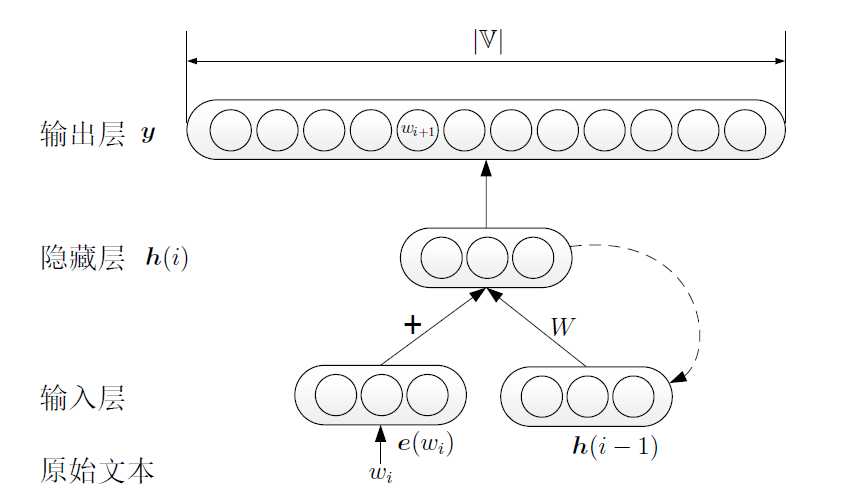
\includegraphics[width=0.7\linewidth]{./figures/rnnlm.png}
  \caption{循环神经网络语言模型(RNNLM)模型结构图}\label{fig:rnnlm}
\end{figure}

RNNLM 的核心在于其隐藏层的算法:
\begin{equation}
\label{equ:rnn}
h_t =\phi(e(w_t) +Wh_{t -1})
\end{equation}
其中,$\phi$非线性激活函数。但与NNLM 不同,RNNLM 并不采用n 元近似,而是使用迭代的方式直接对所有上文进行建模。在公式.~\ref{equ:rnn} 中,h(i) 表示文本中第$i$ 个词$w_i$ 所对应的隐藏层,该隐藏层由当前词的词向量$e(w_i)$ 以及上一个词对应的隐藏层$h(i -1)$ 结合得到。

隐藏层的初始状态为$h(0)$,随着模型逐个读入语料中的词$w_1;w_2; \cdots $, 隐藏层不断地更新为$h(1);h(2); \cdots$ 。根据公式.~\ref{equ:rnn},每一个隐藏层包含了当前词的信息以及上一个隐藏层的信息。通过这种迭代推进的方式,每个隐藏层实际上包含了此前所有上文的信息,相比NNLM 只能采用上文n 元短语作为近似,RNNLM 包含了更丰富的上文信息,也有潜力达到更好的效果。RNNLM 的输出层计算方法与NNLM 的输出层一致。


\section{关键技术或难点}
传统的多元分类模型(Softmax):
\begin{equation}\label{equ:softmax}
  \hat y_i=\frac{\exp(o_i)}{\sum_j \exp(o_j)}
\end{equation}
其中由于分母是正则项,一旦词表扩大,每次迭代更新都需要计算这一项,是主要的问题所在,所以本课题拟在主要解决该问题所导致的计算费时的问题,在保证计算精度不下降的情况下,提高模型的训练速度。目前主要的策略分为: 基于类别的多元分类模型(class-based hierarchical softmax, cHSM)和基于二叉树的二元分类模型(class-based hierarchical softmax, tHSM).

假设语料中的每一个词样本属于且只属于一个类,在此基础上计算词样本在语料中的分布时,可以先计算类的概率分布,然后在所属类上计算当前词的概率分布,于是可将式(3)转化为

\begin{equation}\label{equ:class}
  p(w_i|h_i) = p(c(t)|h(t))p(w_i|c(t))
\end{equation}
此时,训练一个词样本的计算复杂度正比于:$O =HC$. 式中,C 为语料中所有词的分类数,可根据语料中词的词频进行划分. 当C 取1 或取词典大小V 时,此结构等同于标准的RNN 结构. 由于$C \ll V$,通过图1 结构训练的softmax 降低了计算复杂度.

Mikolov曾提出使用基于二叉树的层级softmax模型来加速的训练方案,加速比能达到理论的最大速度,但是当时提出的背景是基于CPU构建的,如今越来越多的算法随着应用领域的推广,需要在并行度更高的GPU上进行计算,因此基于GPU进行建模的tHSM尚未被研究提及,需要后人研讨。


\subsection{关键技术或难点一}
依照上章节的分析,本章节主要介绍我们实验中所要涉及的模型,主要是各种循环神经网络的变种 \cite{DBLP:conf/icml/JozefowiczZS15}: 普通循环神经网络节点、长短记忆网络(Long shrot-term memory, LSTM) \cite{DBLP:journals/taslp/SundermeyerNS15} 和门限记忆节点(Gated Recurrent Unit, GRU) \cite{DBLP:conf/nips/ChungKDGCB15}。 LSTM的计算公式定于如下 \cite{DBLP:journals/neco/HochreiterS97}:
\begin{itemize}
\item 输入门:输入门:控制当前输入 $x_t$ 和前一步输出 $h_{t−1}$ 进入新的 cell 的信息量:$i_t=\sigma(W^i x_t+U^i h_{t-1}+b^i)$
\item  忘记门:决定是否清楚或者保持单一部分的状态$f_t=\sigma(W^f x_t+U^f h_{t-1}+b^f)$
\item  变换输出和前一状态到最新状态$g_t=\phi(W^g x_t+U^g h_{t-1}+b^g)$
\item  输出门: 计算 cell 的输出$o_t=\sigma(W^o x_t+U^o h^{t-1}+b^o)$
\item  cell 状态更新步骤:计算下一个时间戳的状态使用经过门处理的前一状态和输入:$s_t=g_t\odot i_t+s_{t-1}\odot f_t$
\item  最终 LSTM 的输出:使用一个对当前状态的 tanh 变换进行重变换:$h_t=s_t\odot \phi(o_t)$
\end{itemize}
其中$\odot$ 代表对应元素相乘(Element-wise Matrix Multiplication),$\phi(x), \sigma(x)$ 的定义如下:
\begin{equation}\label{equ:tanh}
  \phi(x)=\frac{e^x-e^{-x}}{e^x+e^{-x}},\sigma(x)=\frac{1}{1+e^{-x}}
\end{equation}

\begin{figure}
  \centering
  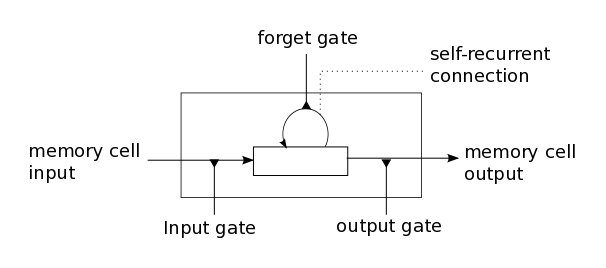
\includegraphics[width=0.7\linewidth]{./figures/lstm_memorycell.png}
  \caption{LSTM 模型}\label{fig:lstm}
\end{figure}


GRU 可以看成是 LSTM 的变种,GRU 把 LSTM中的 forget gate 和 input gate 用 update gate 来替代。 把 cell state 和隐状态 $h_t$ 进行合并,在计算当前时刻新信息的方法和 LSTM 有所不同。 下图是GRU更新 $h_t$ 的过程\cite{DBLP:journals/corr/Pezeshki15}, 具体定义如下:
\begin{itemize}
\item 更新门$z_t$: 定义保存多少以前的信息:$z_t = \sigma ( W^z x_t+ U^z h_{t-1}  )$

\item 重置门$r_t$: 决定保留多少输入信息:$r_t = \sigma(W^r x_t  + U^r h_{t-1}  )$

\item 节点内部更新值$\tilde h_t $: 其次是计算候选隐藏层(candidate hidden layer) $\tilde h_t$,这个候选隐藏层 和LSTM中的$\tilde c_t$是类似,可以看成是当前时刻的新信息,其中$r_t$用来控制需要 保留多少之前的记忆,如果$r_t$为0,那么$\tilde h_t$只包含当前词的信息:$\tilde h_t  = \tanh (W^h x_t  + U^h(h_{t-1} \odot r_t) )$

\item 隐藏层输出值$h_t$: 最后$z_t$控制需要从前一时刻的隐藏层 $h_{t-1}$ 中遗忘多少信息,需要加入多少当前 时刻的隐藏层信息$\tilde h_t$,最后得到$h_t$,直接得到最后输出的隐藏层信息, 这里与LSTM的区别是GRU中没有 输出门:$h_t = (1-z_t)\odot \tilde h_t  + z_t \odot h_{t-1}$
\end{itemize}
如果reset gate接近0,那么之前的隐藏层信息就会丢弃,允许模型丢弃一些和未来无关 的信息;update gate控制当前时刻的隐藏层输出$h_t$需要保留多少之前的隐藏层信息, 若$z_t$接近1相当于我们之前把之前的隐藏层信息拷贝到当前时刻,可以学习长距离依赖。 一般来说那些具有短距离依赖的单元reset gate比较活跃(如果$r_t$为1,而$z_t$为$0$ 那么相当于变成了一个标准的RNN,能处理短距离依赖),具有长距离依赖的单元更新门比较活跃。

\begin{figure}
  \centering
  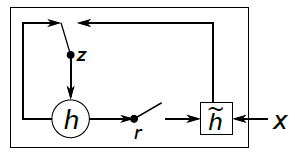
\includegraphics[width=0.5\linewidth]{./figures/gru.png}
  \caption{GRU模型示意图}\label{fig:gru}
\end{figure}


\subsection{关键技术或难点二}
大词表问题,主要是对softmax如何建模的问题。在本课题中,我们探讨cHSM和tHSM两种不同的方案所带来的影响和优劣。
\section{下一阶段工作计划}
当我们使用多层分类模型的时候,我们就需要将单词按照模型的架构进行划分。其中对于cHSM模型,我们有以下策略可以使用:1) 基于词频划分类别 2) 基于2-gram 的布朗聚类(Brown clustering) 进行划分.3)按照word-embedding 的词向量信息进行聚类。另外,我们还需要注意的是,各个类别可以包含不同的数量的单词,也可以包含数量相同的单词。对于后者,我们考虑的划分模型就是基于交换算法(Exchange Algorithm), 以此来保证获得近似的最优解。

\subsection{存在的问题}
\subsection{尚未完成的工作}
\subsection{解决问题的技术思路或措施}
\subsection{下一阶段计划}
\begin{itemize}
  \item 2017年8月 $\sim$ 2017年9月: 继续整理资料,学习研究语言模型和循环神经网络的领域知识;
  \item 2017年9月 $\sim$ 2017年10月: 继续研究学习深度学习模型在语言模型上是如何使用的过程;
  \item 2017年10月 $\sim$ 2017年11月: 继续调研并实现解决大词表问题的主要手段, 并完善基本代码框架;
  \item 2017年11月 $\sim$ 2017年12月: 补充完整实验验证与完善;
  \item 2017年12月 $\sim$ 2018年1月: 资料整理和论文撰写.
\end{itemize}


1) 数学背景和理论背景。 尽管本实验题目定义范围比较小,但是我们也需要很好的数学理论知识,包括:矩阵论,概率论。还有,我们还需要极强的阅读外文文献知识和编码实现能力,都是不可或缺的基本要求。

2) 基于theano框架的建模方案。因为基于 python 的深度学习库比较完善,适合建模。 本实验拟采用 theano 的建模语言,来帮助我们快速建模和调参。Theano是在BSD许可证下发布的一个开源项目,是由LISA集团(现MILA)在加拿大魁北克的蒙特利尔大学(Yoshua Bengio领导的实验室)开发。它是用一个希腊数学家的名字命名的。Python的核心Theano是一个数学表达式的编译器。它知道如何获取你的结构,并使之成为一个使用numpy、高效本地库的非常高效的代码,如BLAS和本地代码(C++),在CPU或GPU上尽可能快地运行。它巧妙的采用一系列代码优化从硬件中攫取尽可能多的性能。如果你对代码中的数学优化的基本事实感兴趣,看看这个有趣的名单。Theano表达式的实际语法是象征性的,可以推送给初学者用于一般软件开发。具体来说,表达式是在抽象的意义上定义,编译和后期是用来进行计算。它是为深度学习中处理大型神经网络算法所需的计算而专门设计的。它是这类库的首创之一(发展始于2007年),被认为是深度学习研究和开发的行业标准。

3) 同时本实验也需要对linux的bash脚本有一定的熟悉,以方便将模型的数据结果正确的统计和运行模型的开发环境配置。

4) 试验结果图表统计和绘制.本实验的结果需要精良的语言来控制,而R语言的ggplot2框架就很适合我们的试验结果图表的绘制工作。

5) 基于GPU的cuda的模型优化也是我们需要考虑的问题之一。CUDA技术有下列几个优点:1) 分散读取,代码可以从内存的任意位址读取; 2)共用内存,CUDA公开一個快速的共用存储区域(每个处理器48K),使之在多个进程共用。同时他的缺点可以归纳为: 1) CUDA不支持完整的C语言标准。它在C++编译器上运行代码时,会使一些在C中合法(但在C++中不合法)的代码无法编译; 2) 双精度浮点与IEEE754标准有所差异:倒数、除法、平方根僅支持舍入到最近的偶数。单精度中不支持反常值(denormal)及sNaN(signaling NaN);只支持两种IEEE舍入模式(舍位与舍入到最近的偶数),这些在每条指令的基础上指定,而非控制字码;除法/平方根的精度比单精度略低。



\newpage
\addcontentsline{toc}{section}{主要参考文献}
\buaathesisbib{bibs}

\end{document}
